\section{Results}
\label{sec:analysis}

Our experiments reveal that the learning strategies adopted by Transformers are systematically shaped by the predictability of their training environment, in ways that closely parallel adaptive mechanisms in evolutionary biology.
We first examine how environmental stability and cue reliability governs the asymptotic preference for ICL versus IWL. We then explore the learning dynamics between these strategies, revealing task-dependent patterns of transience (ICL $\to$ IWL and vice versa). Finally, we show that the cost of acquiring ICL versus IWL governs these dynamics. Together, these results reconcile a diverse set of learning phenomena in Transformers with
principles of biological adaptation.

\begin{figure}[!ht]
  \centering
  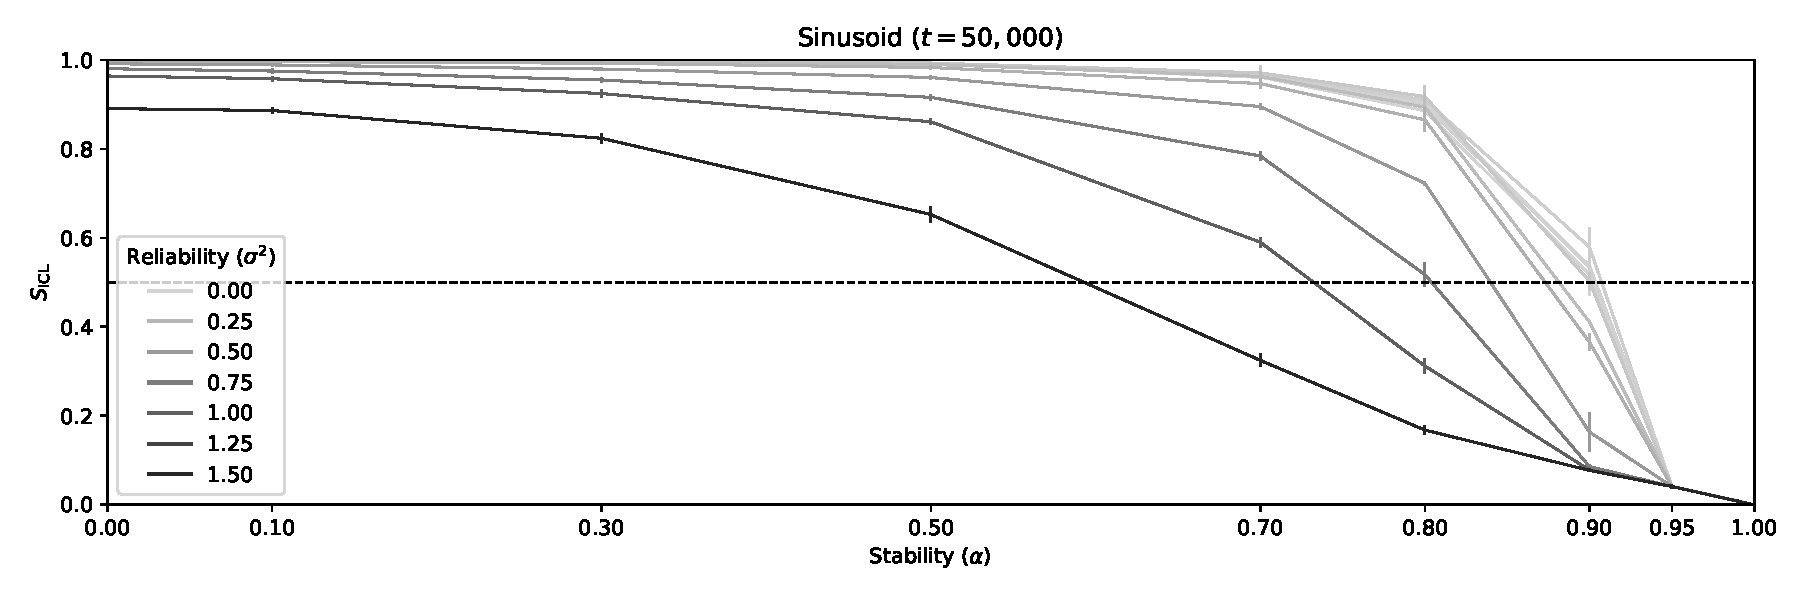
\includegraphics[width=0.99\linewidth]{figures/sinusoid_asymptotic.pdf}
  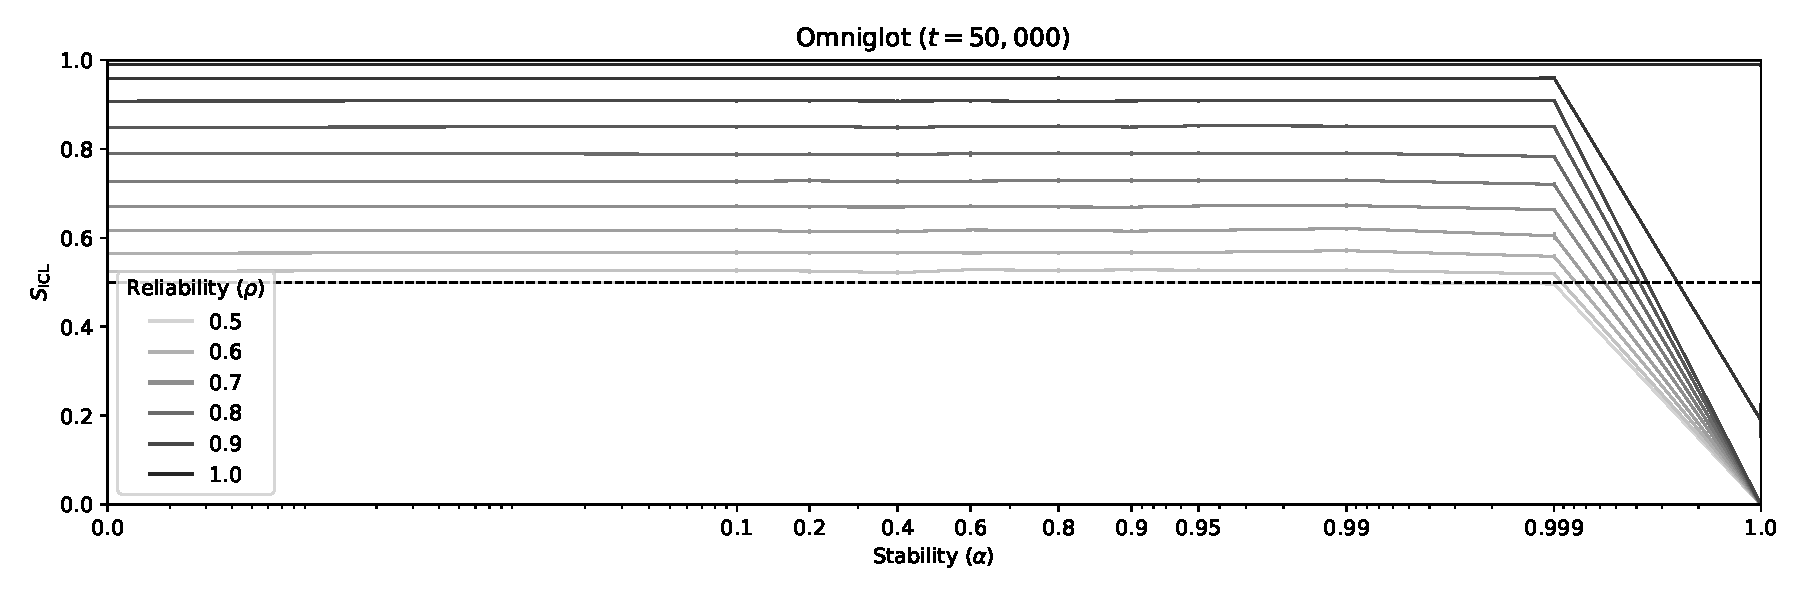
\includegraphics[width=0.99\linewidth]{figures/omniglot_asymptotic.pdf}
  \caption{
    The asymptotic strategy of converged models ($t = 50,000$).
    The ICL preference score ($S_\text{ICL}$) is plotted as a function of environmental stability (x-axis) and cue reliability (line brightness).
    The dashed line at $S_\text{ICL} = 0.5$ marks the crossover point.
    In sinusoid regression (top), stability is parameterized by the AR(1) coefficient $\alpha$. Cue reliability increases with decreasing noise variance $\sigma^2$ (lighter lines).
    In Omniglot classification (bottom), stability is parameterized by the mapping persistence $\alpha$ (logit scale). Cue reliability increases with label correctness probability $\rho$ (lighter lines).
  }
  \label{fig:asymptotic}
\end{figure}

\subsection{Determinants of asymptotic strategy}
\label{sec:asymptotic}

Figure~\ref{fig:asymptotic} shows how dimensions of environmental predictability influence the model's asymptotic strategy ($t = 50,000$), supporting our core hypothesis that information reliability across timescales governs the trade-off between ICL and IWL.

\textbf{Stable environments favor ICL.}
In sinusoid regression (Figure~\ref{fig:asymptotic}, top), increasing environmental stability ($\uparrow\alpha$) leads to a precipitous decline in ICL preference. As $\alpha \to 1$, the model shifts almost entirely to IWL. This recapitulates the biological principle of genetic assimilation: when environmental features are stable across generations, selection favors the permanent encoding of traits over incurring cost of plasticity \cite{stearns1989evolutionary,dewitt1998costs}. Similarly, in the Omniglot task (Figure~\ref{fig:asymptotic}, bottom), ICL preference plummets as $\alpha \to 1$. This reflects a transition where the global mapping becomes invariant, allowing the model to consolidate the task into its weights and render the prompt redundant.

\textbf{Volatile environments with reliable cues favor ICL.}
Conversely, when environmental stability is low, the model relies heavily on ICL, provided that reliable cues are available. In sinusoid regression, reliable cues ($\downarrow\sigma^2$, lighter lines) fosters strong ICL preference. This aligns with the evolutionary view that plasticity is favored specifically when environmental fluctuations render fixed traits maladaptive, but only if accurate cues exist to guide the plastic response \cite{stephens1989variance,scheiner1993genetics}.
In Omniglot, this effect is even more pronounced: across a broad range of instability ($\alpha < 0.95$), cue reliability is the primary determinant of strategy.

\textbf{When strategies are equally effective.}
Interestingly, we observe a deviation from biology in the Omniglot task. With perfectly reliable cues ($\rho = 1$), the model maintains a strong preference for ICL even when the environment is perfectly stable (Figure~\ref{fig:asymptotic}, bottom right). Evolutionary theory suggests that plasticity is selected against in stable environments due to maintenance costs \cite{dewitt1998costs}. The persistence of ICL here implies that, for Transformers, the maintenance cost of ICL may be negligible --- or, crucially, that the acquisition cost of the alternative strategy (IWL) is prohibitively high. This suggests that when both strategies are asymptotically effective, the model's preference is driven by the difficulty of learning each solution. We formalize this intuition in Section~\ref{subsec:relative_cost_hypothesis}.

\begin{figure}[!ht]
  \centering
  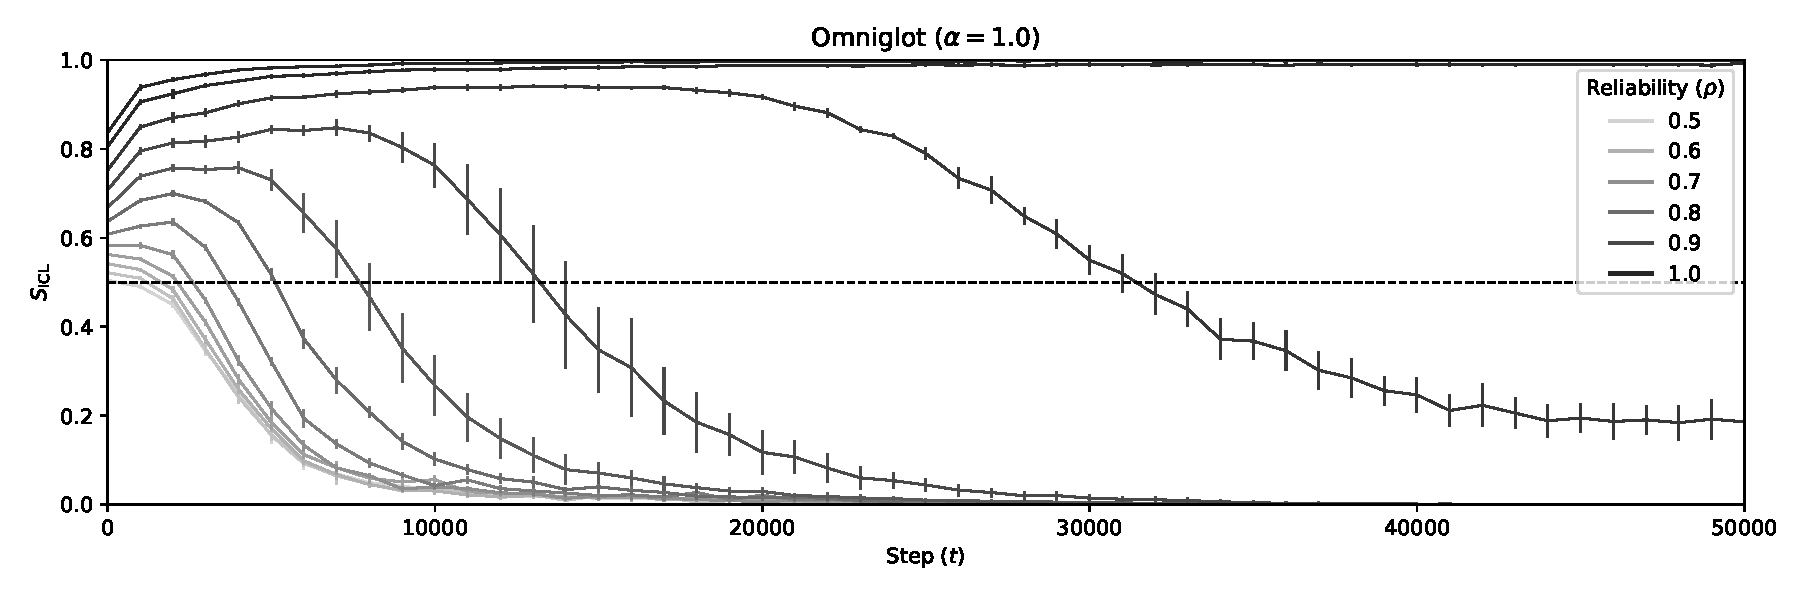
\includegraphics[width=0.99\linewidth]{figures/omniglot_transience.pdf}
  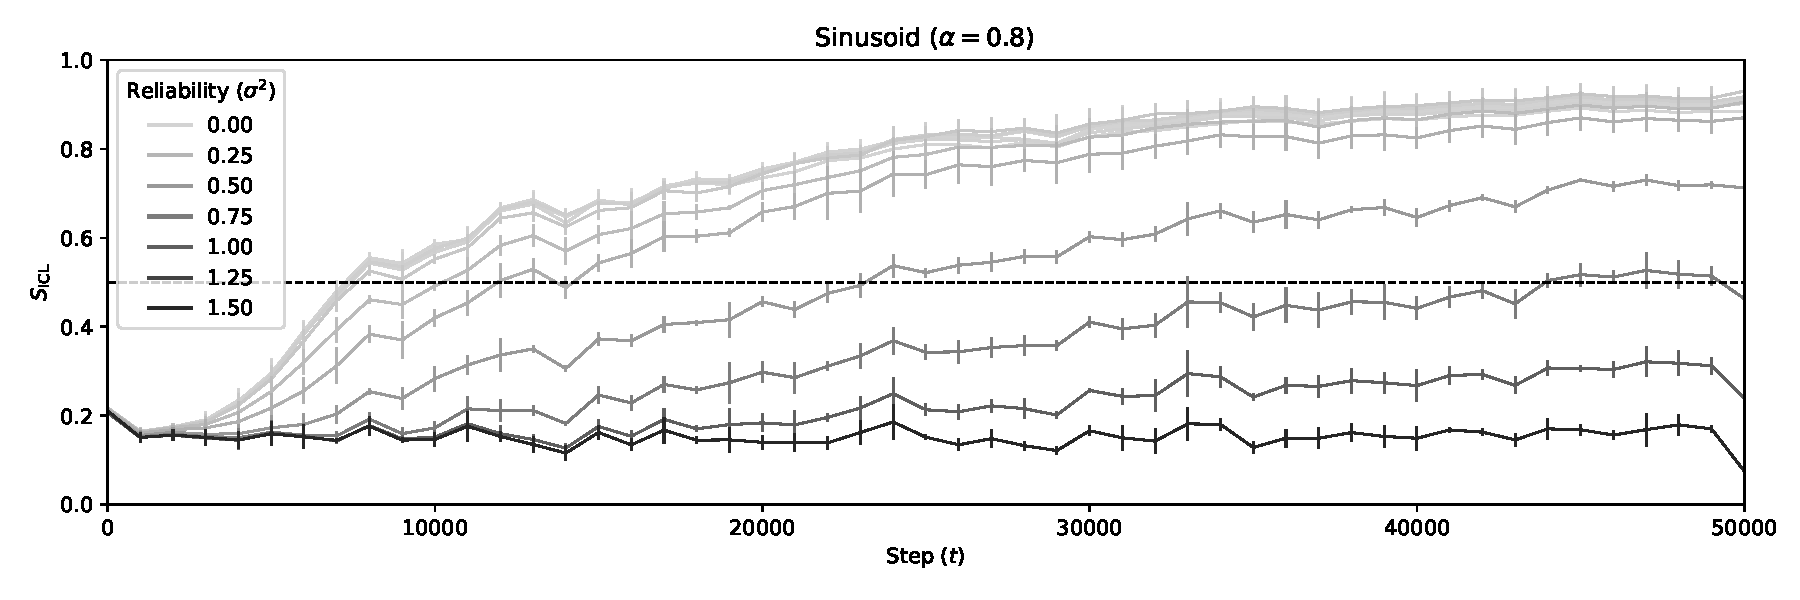
\includegraphics[width=0.99\linewidth]{figures/sinusoid_transience.pdf}
  \vspace{-0.5em}
  \caption{
  % Learning dynamics and transience.
  The shift in ICL preference ($S_\text{ICL}$) over training steps ($t$) reveals opposing directions of transience. Omniglot classification (top) demonstrates ICL transience ($\alpha=1$). The model initially relies on ICL but gradually consolidates the task into weights. Sinusoid regression (bottom) demonstrates IWL transience ($\alpha=0.8$). The model initially relies on IWL but gradually improves inferences by using the prompt.
  }
  \label{fig:transience}
\end{figure}

\subsection{Task-dependent patterns of transience}
\label{sec:transience}

Beyond asymptotic strategies, the learning trajectories reveal shifts in strategy preference during training --- a phenomenon known as \textit{transience} \cite{singh2023transient,panwar2023context,singh_strategy_2025}. As shown in Figure~\ref{fig:transience}, the direction of change between ICL and IWL is highly task-dependent.

\textbf{ICL transience (ICL $\to$ IWL).} In the Omniglot task under high environmental stability (Figure~\ref{fig:transience}, top), we observe the phenomenon of ICL transience \cite{singh2023transient}. The model exhibits a strong preference for ICL early in training. However, as training progresses, the model gradually shifts towards an IWL solution. This progression parallels genetic assimilation, where a trait initially induced by environmental cues (plasticity) becomes genetically encoded under prolonged, stable selection, eventually rendering the cue redundant \cite{waddington1953genetic, pigliucci2006phenotypic}.

\textbf{IWL transience (IWL $\to$ ICL).} In contrast, the sinusoid regression task (Figure~\ref{fig:transience}, bottom) exhibits the opposite trajectory: IWL transience (or delayed ICL). Under medium stability ($\alpha=0.8$), the model initially relies on IWL (approximating the function via weights) and exhibits a low preference for context. A strong preference for ICL emerges only later in training, particularly when cues are highly reliable ($\downarrow\sigma^2$). This suggests that for sinusoid regression, an IWL approximation of the target function is easier to learn early on, whereas the circuitry required for ICL develops more slowly. This pattern relates to phenomena like \textit{grokking}, where generalization capability (here, ICL) emerges abruptly after a long period of fitting the training distribution \cite{power2022grokking}.

\subsection{Cost-based arbitration between strategies}
\label{subsec:relative_cost_hypothesis}

The contrasting trajectories observed in Section~\ref{sec:transience} raise the question of why Transformers initially prefer ICL in Omniglot (ICL $\to$ IWL), but IWL in Sinusoid (IWL $\to$ ICL). These results suggest that learning dynamics are governed not only by the asymptotic optimality of a strategy (which is determined by the environment), but also by the cost of acquiring that strategy. We posit that the strategy that is cheaper to learn (i.e., whose inductive bias closely fits the task structure) will emerge earlier in training, regardless of whether it is the long-term optimal solution.
This aligns with the broader literature on \textit{simplicity bias}~\cite{arpit2017closer,goldblum2023no,deora2025context}, while highlighting that simplicity is contingent on the correspondence between the model and the training data.

\textbf{Cost of learning for each strategy.}
Intuitively, the relative difficulty of IWL and ICL differs across our two tasks.
In Omniglot, IWL requires memorizing a global mapping for a large vocabulary ($|\mathcal{C}| = 1623$). This is a high-capacity memorization problem with high sample complexity. In contrast, ICL requires only a local pattern-matching circuit (comparing the query to the prompt) \cite{olsson2022context, singh_what_2024}, which is simple for the attention mechanism to discover. Thus, for Omniglot, ICL is cheaper than IWL.
In sinusoid regression, the dynamic is reversed. An IWL solution requires learning a single global sine wave approximation, which neural networks can parameterize rapidly. Conversely, ICL requires implementing a regression algorithm within the forward pass (e.g., gradient descent or ridge regression via attention \cite{von2023transformers}). This is a complex circuit that is difficult to learn. Thus, for sinusoid, IWL is cheaper than ICL.

\textbf{Quantifying learning cost.} To formalize this intuition, we adopt the minimum description length (MDL) perspective for quantifying the cost of learning a particular dataset, using the \textit{prequential codelength} \cite{blier2018description}.
Prequential codelength is the cumulative negative log-likelihood (NLL) of each token, computed sequentially by a model strategy (ICL or IWL) trained on all preceding tokens. See Appendix~\ref{sec:prequential} for a formal description. Intuitively, a strategy that is easier to learn for the particular dataset (more aligned inductive bias) will achieve lower log-likelihoods early in training, resulting in a shorter prequential codelength.\footnote{Prequential codelength also exhibits a ``catch-up phenomenon'' that may be interesting to compare with our transience observations here --- complex models have higher cost initially and later require more samples to ``catch up'', even after they become more optimal \cite{erven_catching_2012}.}

Because our goal is to evaluate the inductive bias of different learning strategies the transformer can adopt (ICL or IWL), rather than the Transformer as a whole, we consider training environments where either ICL or IWL are strongly favored. For ICL, this means a volatile environment ($\alpha=0.0$) with reliable cues ($\rho=1.0, \sigma^2=0.0$). And for IWL, this means a stable environment ($\alpha=1.0$) with unreliable cues ($\rho=0.5, \sigma^2=1.5$). We then computed the prequential codelength of each strategy (ICL and IWL) for each task (sinusoid and Omniglot) by keeping a running sum of the NLL (i.e., the loss) during the entire course of training.\footnote{It is worth noting that for the Omniglot task, the binary cross-entropy loss is equivalent to the NLL; however for sinusoid regression, the mean squared error loss is monotonically related to the NLL under a Gaussian likelihood.}
As shown in Figure~\ref{fig:coding_cost}, the results confirm our intuition. For Omniglot, the cost for ICL is significantly lower than for IWL. Conversely, for sinusoid, the cost for IWL is significantly lower than for ICL. This metric predicts the starting point of the learning trajectories in Figure~\ref{fig:transience} --- the model adopts the cheaper strategy first.

\begin{figure}[!ht]
  \centering
  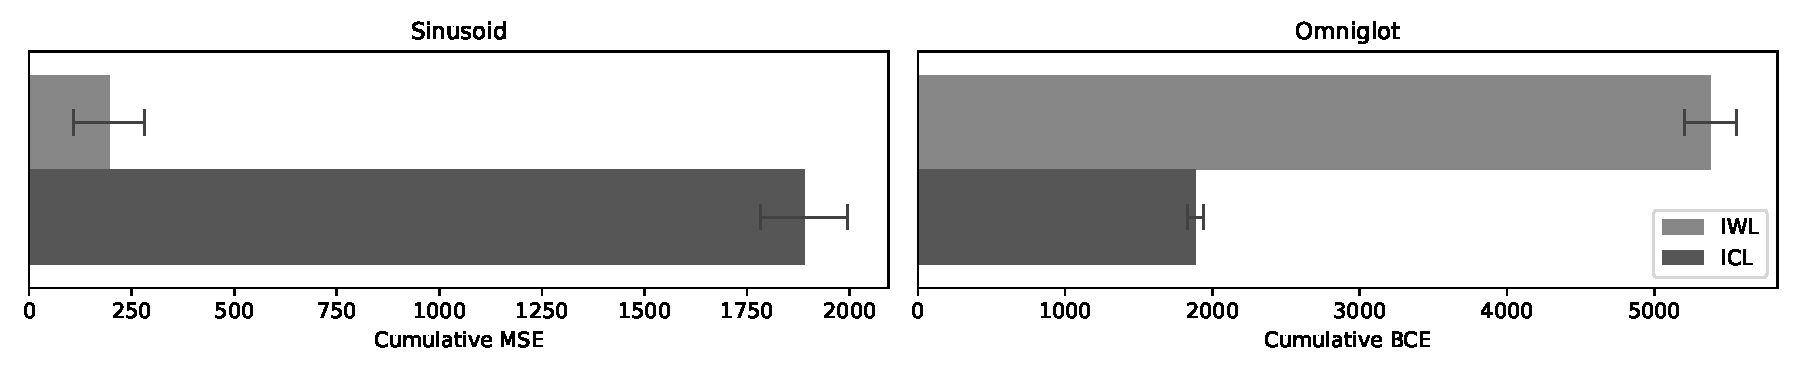
\includegraphics[width=0.99\linewidth]{figures/coding_cost.pdf}
  \caption{Cost of learning IWL vs ICL, measured as the prequential codelength (cumulative MSE/BCE loss accrued over 50,000 training steps). IWL is less expensive than ICL for Sinusoid, and the reverse is true for Omniglot, showing that the relative cost of IWL vs ICL corresponds to transience dynamics (IWL-first or ICL-first) observed experimentally for the two tasks.}
  \label{fig:coding_cost}
\end{figure}


\textbf{Manipulating learning cost.}
To causally validate that learning cost drives these dynamics, we manipulated the difficulty of the IWL strategy in the Omniglot task. The sample complexity of IWL (memorizing labels for all characters) is governed by the coupon collector problem --- to see all $N=|\mathcal{C}|$ characters at least $K$ times requires $\Theta(KN \log N)$ episodes. By reducing the vocabulary size $|\mathcal{C}|$, we reduce the cost of the IWL strategy.

As Figure~\ref{fig:reversal} shows, reducing $|\mathcal{C}|$ from 1623 to 100 drastically changes the learning dynamics. In the standard setting (dark line), the model starts with high ICL preference. However, in the reduced setting (lightest line), the dynamics reverse: the model starts with a preference for IWL ($S_\text{ICL} < 0.2$) before eventually switching to ICL. This induced IWL transience (reproducing the dynamic seen in the Sinusoid task) shows that the initial preference of a strategy is determined by its acquisition cost.

\begin{figure}[!ht]
  \centering
  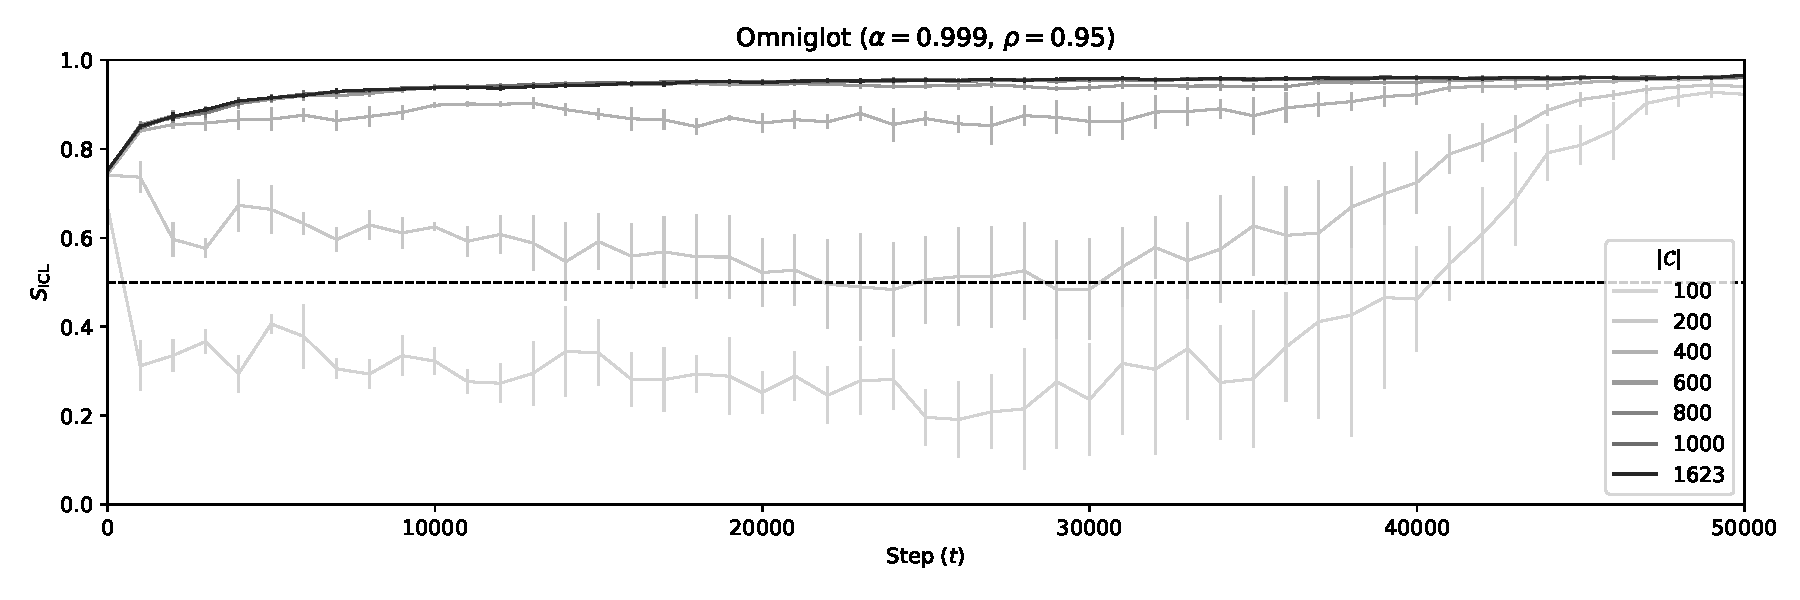
\includegraphics[width=0.99\linewidth]{figures/omniglot_reversal.pdf}
  \caption{
    % \textbf{Causal validation of acquisition cost.}
    We manipulate the learning cost of the IWL strategy by varying the Omniglot vocabulary size ($|\mathcal{C}|$).
    We plot ICL preference ($S_\text{ICL}$) across training steps ($t$) in a stable environment ($\alpha=0.999$) with reliable cues ($\rho=0.95$).
    In the standard setting ($|\mathcal{C}|=1623$, dark line), the model exhibits a sustained preference for ICL.
    Drastically reducing the vocabulary size (e.g., to $|\mathcal{C}|=100$, lightest line) lowers the cost of IWL, causing the model initially favors IWL before eventually switching to ICL, thereby reversing the pattern of transience previously observed in this task.
  }
  \label{fig:reversal}
\end{figure}


Our findings align with recent work linking ICL transience to task structure \cite{singh2023transient} and relative acquisition speeds \cite{nguyen_differential_2024,singh_strategy_2025,wurgaft2025context}, as well as mechanistic studies on circuit efficiency  and competition dynamics \cite{thilak_slingshot_2022, nanda_progress_2023, varma_explaining_2023,park2024competition}. Together, they imply that Transformers arbitrate between strategies based on a distinct optimization cost. The framework of {\em resource rational analysis} \cite{lieder2020resource}, introduced in cognitive science but inspired by earlier work in AI \cite{horvitz1987reasoning,russell1994provably}, may provide a set of tools for formalizing this tradeoff and offering further insight into the behavior of AI models. 
